%	!Mode::"UTF-8"
%	本模板设置改自北京大学交叉学院 王宇哲学长和北京大学化学与分子工程学院 王应泽同学的分享,特此感谢!
%	模板制作:北京大学化学与分子工程学院 王梓涵
%	Email:2100011837@stu.pku.edu.cn
%	本模板仅适用于北京大学物理化学实验报告,其他学校请自行修改
%	吐槽:Latex用于写物化实验报告还是过于繁琐了,不过还是比Word好用多了(๑•̀ㅂ•́)و✧ (此吐槽由copilot自动生成,模板作者认为word更好用)
%	本模板仅供交流学习使用,不可用作商业用途。

\documentclass[12pt]{article}

%	页面设置
\usepackage{geometry}
\geometry{left=2.5cm, right=2.5cm, top=2.5cm, bottom=2.5cm}
\usepackage{graphicx}
\usepackage{ctex}
\usepackage{fontspec}
\usepackage{setspace}
\usepackage[usenames,dvipsnames]{xcolor}
\usepackage{titlesec}

%	字体设置
\setmainfont{Times New Roman}
\setCJKmainfont{SimSun}
\setCJKsansfont{SimHei}
\setCJKmainfont[AutoFakeBold=true]{SimSun}

%	表格设置\
\usepackage{array,colortbl}
\usepackage{makecell}
\newcommand{\addcell}[2][4]{\makecell{\zihao{#1}\textsf{#2}}}
\usepackage{titlesec}
\usepackage{booktabs}
\usepackage{ragged2e} 
\usepackage{multirow}
\usepackage{tabularx}

%	设置图注、表注
\usepackage{caption}
\usepackage{bicaption}
\captionsetup{labelsep=quad, font={small, bf}, skip=2pt}
\DeclareCaptionOption{english}[]{
    \renewcommand\figurename{Fig.}
    \renewcommand\tablename{Table}
}
\captionsetup[bi-second]{english}

%	设置页眉
\usepackage{fancyhdr}
\usepackage{xpatch}
\pagestyle{fancy}
\fancypagestyle{preContent}{
    	\fancyhead[L]{\zihao{-5} 物理化学实验}
    	\fancyhead[C]{\zihao{-5} 实验二\ \ 燃烧热的测定}
    	\fancyhead[R]{\zihao{-5} 2100011837\ 王梓涵}
		\renewcommand{\headrulewidth}{2pt}
		\renewcommand{\footrulewidth}{1pt}
		\xpretocmd\headrule{\color{BrickRed}}{}{\PatchFailed} % 设置页眉分割线颜色
		\xpretocmd\footrule{\color{BrickRed}}{}{\PatchFailed} % 设置页脚分割线颜色
}
\pagestyle{preContent}



%	设置首页页眉及取消首页页脚 若不需要首页页眉 请注释掉下列内容
\fancypagestyle{plain}{
	\fancyhead[L]{\zihao{-5} 物理化学实验}
    \fancyhead[C]{\zihao{-5} 实验二\ \ 燃烧热的测定}
	\fancyhead[R]{\zihao{-5} 2100011837\ 王梓涵}
	\cfoot{}
}

%	设置标题格式
\titleformat*{\section}{\color{Mahogany}\zihao{4}\sffamily}
\titleformat*{\subsection}{\zihao{-4}\sffamily}
\titleformat*{\subsubsection}{\zihao{-4}\sffamily}
\titlespacing*{\section}{0pt}{10pt}{10pt}
\titlespacing*{\subsection}{0pt}{10pt}{5pt}
\titlespacing*{\subsubsection}{0pt}{10pt}{5pt}


%	设置引用格式(ACS格式规范)
%	注意:请安装JabRef
%	JabRef使用参考:https://blog.csdn.net/weixin_44191286/article/details/85698921
\usepackage[super,round,comma,compress]{natbib}

%	数学公式增强
\usepackage{amsmath}
\usepackage{amssymb}
\usepackage[version=4]{mhchem}
\usepackage{mathtools}
\usepackage{diffcoeff}

%	单位与数学式
\usepackage{siunitx}

%	设置封面
\begin{document}
    % 标题页
    \begin{titlepage}
    	% 页眉
    	\thispagestyle{plain}
        % 校徽图片
        \begin{figure}[h]
            \centering
            \includegraphics{pku.png}
        \end{figure}
        \vspace{24pt}
        % 标题
        \centerline{\zihao{-0} \textsf{\textcolor{Mahogany}{物理化学实验报告}}}
        \vspace{40pt} % 空行
        \begin{center}
            \begin{tabular}{cp{14.1cm}}
                % 题目
                \addcell[2]{题目:} & \addcell[2]{燃烧热的测定} \\
                \cline{2-2}
            \end{tabular}
        \end{center}
        \vspace{20pt} % 空行
        \begin{center}
            \doublespacing
            \begin{tabular}{cp{5cm}}
                % 姓名
                \addcell{姓\phantom{空格}名:\ } & \addcell{王梓涵} \\
                \cline{2-2}
                % 学号
                \addcell{学\phantom{空格}号:\ } & \addcell{2100011837}\\
                \cline{2-2}
                % 组别
                \addcell{组\phantom{空格}别:\ } & \addcell{22组} \\
                \cline{2-2}
                % 实验日期
                \addcell{实验日期:\ } & \addcell{2023.12.14}\\
                \cline{2-2}
                % 室温
                \addcell{室\phantom{空格}温:\ } & \addcell{289.95\ K}\\
                \cline{2-2}
                % 大气压强
                \addcell{大气压强:\ } & \addcell{99.45\ kPa}\\
                \cline{2-2}
            \end{tabular}
            \begin{tabular*}{\textwidth}{c}
                \\ % 这是空行
                \\ % 这是空行
                \\ % 这是空行
                \hline % 分割线
            \end{tabular*}
        \end{center}
        % 摘要
        \textsf{\textcolor{BrickRed}{摘\ \ 要}}\ \  本实验通过氧弹式量热计中苯甲酸、蔗糖和单晶冰糖的恒容燃烧,经雷诺校正及热力学计算得到量热计常数$W=(2.243\pm 0.097)\ \ {\rm kJ\cdot K^{-1}}$,单晶冰糖的恒压燃烧热$Q_{V}=-(1.684\pm 0.070)\times 10^{4}\ \ {\rm kJ\cdot g^{-1}}$,恒容燃烧热$Q_{P}=-(1.684\pm 0.070)\times 10^{4}\ \ {\rm kJ\cdot g^{-1}}$,与文献值的偏差$\xi=2.2\%$,使用 Origin 软件进行雷诺校正,测得样品白方糖燃烧热$Q_{P}=Q_{V}=-(1.538\pm 0.107)\times 10^{4}\ \ {\rm kJ\cdot g^{-1}}$。
        \\
        \\
        % 关键字
        \textsf{\textcolor{BrickRed}{关键词}}\ \ 燃烧热;氧弹式热量计;雷诺校正
    \end{titlepage}

    \section{引言}
		\subsection{实验目的}
			本实验的实验目的主要有以下几点\citealp{physchemlab}:\par
			\ \ \ \ \ \ \ \ 1. 了解热量计的原理、构造和使用方法。\par
			\ \ \ \ \ \ \ \	2. 进行有关热化学实验的一般知识和基本训练。\par

		\subsection{实验原理和实验方法}
		本实验使用氧氮式热量计计算燃烧过程的热效应,具体的实验原理和实验方法在实验预习报告中如\textbf{图1}所示: \par
		\begin{figure}[h]
			\centering
			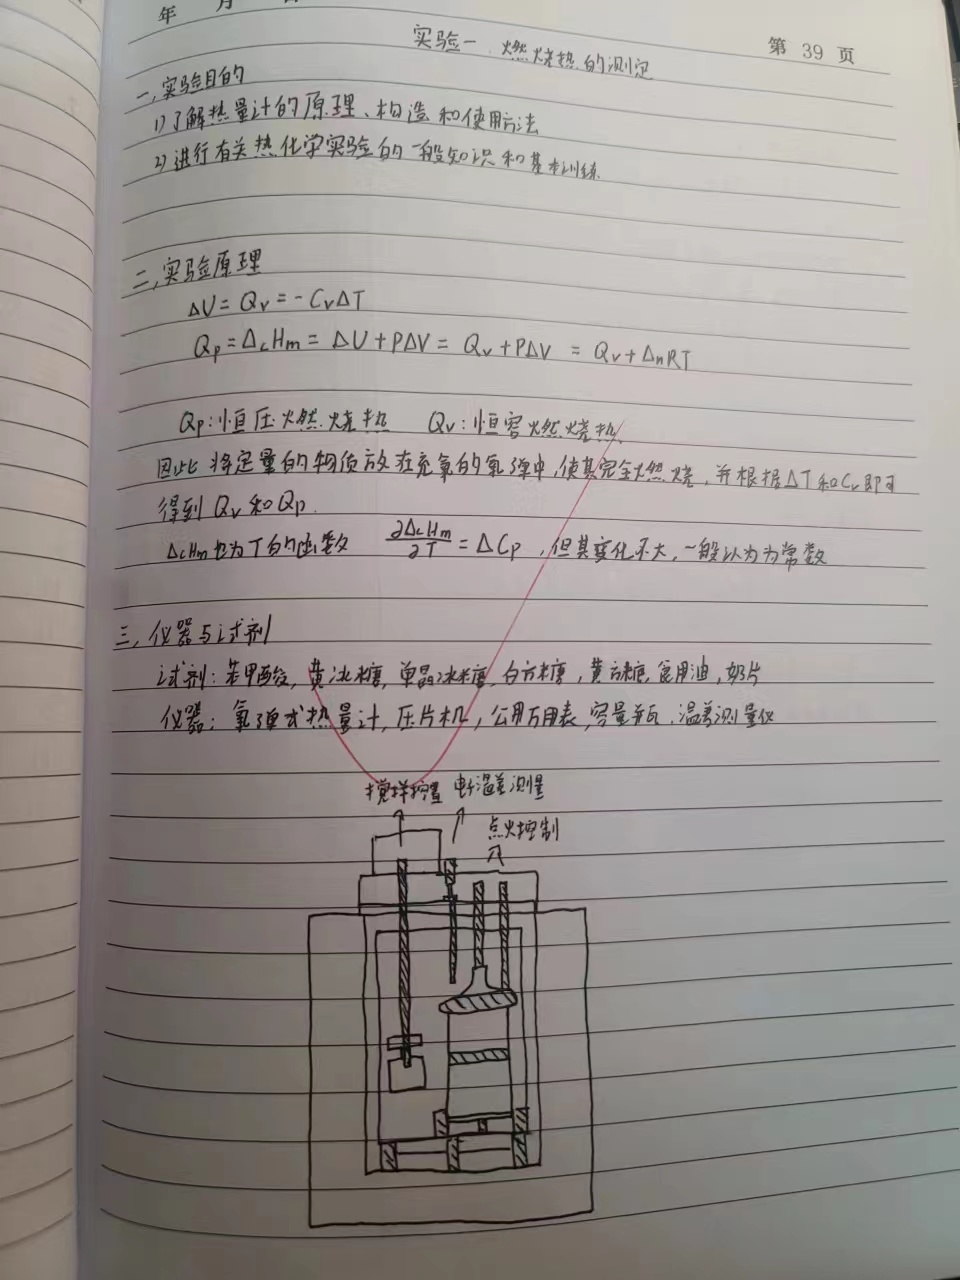
\includegraphics[width=0.6\textwidth]{1.png}
			\bicaption{实验预习报告的实验原理部分}{The principle part of the experiment in the experiment preview report}
		\end{figure}
			
	     
    \section{实验部分}
    	\subsection{仪器和试剂}
    		仪器:氧弹式量热计,氧气钢瓶,压片机,温差测量仪,容量瓶,共用万用表,研钵及研杵 \par
			试剂:苯甲酸(AR),蔗糖(AR),去离子水,单晶冰糖。\par
    			
    	 \subsection{实验内容}
		 本实验采用面向过程的指导型探究学习(POGIL)教学方法,包含两轮“实验操作——现象与数据分析——思考与讨论”环节。
		 本实验的实验操作如下所示,其中笔者的思考和具体实验中的不同操作会在括号中写出。\par
		 \subsubsection{第一轮实验(预实验)}
		 \textbf{探究问题}:一克蔗糖会使热量计体系升温多少度?\par
		 \textbf{1.} 取0.0275 g 棉线,并用其绑住一块约0.5 g 的蔗糖,棉线与蔗糖总重0.6044 g。取 0.0074 g 镍丝,将两端与电极连接,拧紧螺母固定。将样品系在镍丝上,挂在燃烧皿中。\par
		\textbf{2.} 盖好弹盖,灌入 1.0 MPa 氧气。使用万用表测定弹头及进气阀体间电阻,约为 $ 3.77\ \ \Omega$,\textbf{(实际测量时数值波动较大,在 $3.20 \sim 7.50\ \ \Omega$之间)。}\par
		\textbf{3.} 定容 3000 mL 去离子水,小心加入内筒。将氧弹放入内筒中,盖上盖板,插入温差仪探头,开启搅拌马达。待水温稳定后,使用软件开始记录数据。保证记录平台期 120 s后,按住点火键约 3 s 点燃样品,体系温度迅速上升。待温度平稳后,继续记录 120 s。后停止搅拌,取出温差仪探头,取出氧弹,在通风橱中卸去废气。取出弹头,称取镍丝残余质量为 0.0048 g\textbf{(实际测量过程中,因为镍丝被烧断,引起无法保证称量的镍丝就是全部剩余的镍丝)}。燃烧皿底部残留少量黑色物质。\par


		\subsubsection{第二轮实验(利用苯甲酸标样测定仪器水当量)}
		\textbf{探究问题}:如何测量水的当量?\par
		\textbf{1.} 倒出量热仪中的水,擦干氧弹内外部,重新定容 3000 mL 并加入。粗称约 0.85 g 苯甲酸样品,压制成圆柱形。取 0.0262 g 棉线,系住圆柱形苯甲酸样品,再次称量苯甲酸及棉线总重,为 0.8672 g。\par
		\textbf{2.} 称取 0.0095 g 镍丝,类似 \textbf{2.2.1} 中操作,连接电极,悬挂样品。经讨论,大气中存在 $N_{2}$,可能生成其他产物(如生成 $NO_{2}$,与水结合生成硝酸),可能对燃烧热测定产生影响。因此此次测定首先充放氧气三次,再充氧气 1.0 MPa。测定电阻约为$ 4.72\ \ \Omega$。\par
		\textbf{3.} 类似 \textbf{2.2.1}中操作,测定温度-时间曲线。测定完毕后称量残余镍丝质量为 0.0021 g。燃烧皿底部及边沿有少量黑色物质残余。

		\subsubsection{第三轮实验(测定单晶冰糖的燃烧热)}
		\textbf{1.} 倒出量热器中的水,擦干氧弹内外,重新定容 3000 mL 水并加入内筒。类似 \textbf{2.2.1}中测定过程,称取棉线 0.0192 g,棉线及冰糖总重 1.7283 g,镍丝 0.0096 g。氧弹充放气三次,后充入 1.0 MPa 氧气。\par
		\textbf{2.} 重复\textbf{2.2.1}和\textbf{2.2.2}中的类似步骤,测定温度-时间曲线。测定完毕后称取残余镍丝质量为 0.0043 g。\par
	 \section{数据与结果}
 		\subsection{实验数据记录及处理}
 			\subsubsection{第一轮实验}
			测定蔗糖燃烧温差-时间关系如\textbf{图2}所示。
			\begin{figure}[h]
				\centering
				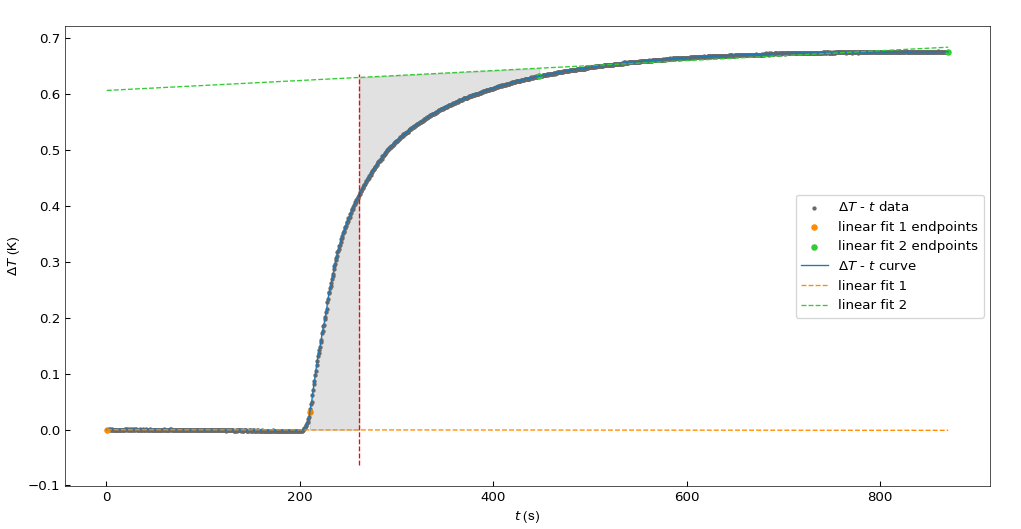
\includegraphics[width=0.9\textwidth]{2.png}
				\bicaption{蔗糖燃烧温差-时间关系}{The relationship between the temperature difference and time of sucrose combustion}
			\end{figure}
			读取原始数据,燃烧前平台期温度 T1 = -0.001 K,燃烧后平台期温度为 T2 = 0.630 K。称取蔗糖质量为 0.5769 g。可据此计算每克蔗糖引起体系温升值:、
			\begin{equation}
				\Delta T = \frac{T_{2}-T_{1}}{m_{s}} = \frac{0.630+0.001}{0.5769} = 1.091\ \ {\rm K\cdot g^{-1}}
			\end{equation}
			\par
			可以注意到,蔗糖燃烧后,燃烧皿底部残留少量黑色物质,这可能是蔗糖燃烧产生的碳残留。\par

			\subsubsection{第二轮实验}
			苯甲酸样品燃烧过程温差-时间关系图如\textbf{图3}所示。测定时室温为 289.45 K。\par
			\begin{figure}[h]
				\centering
				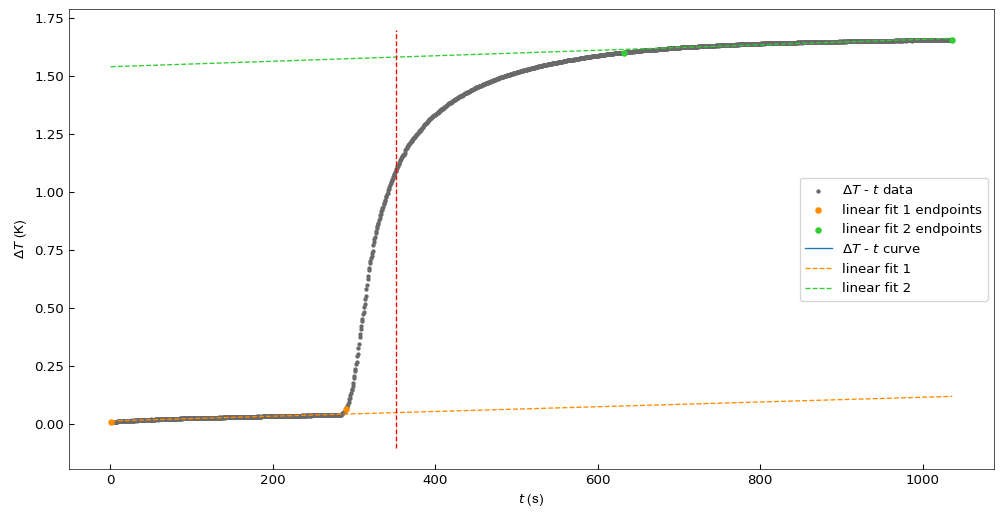
\includegraphics[width=0.9\textwidth]{3.png}
				\bicaption{苯甲酸燃烧温差-时间关系}{The relationship between the temperature difference and time of benzoic acid combustion}
			\end{figure}
			由平台进行雷诺矫正后可知,燃烧前平台期温度 T1 = 0.049 K,燃烧后平台期温度为 T2 = 1.581 K。因此燃烧前后的温差:
			\begin{equation}
				\Delta T = T_{2}-T_{1} = 1.581-0.049 = 1.532\ \ {\rm K}
			\end{equation}
			仪器的量热器常数(水当量)$W$可由下式求算:
			$$
			W=\frac{-Q_{V}G-\Sigma q}{\Delta T_{0}}-DC_{\rm H_{2}O}
			$$
			\par
			其中$G$为苯甲酸的质量,由\textbf{2.2.2}知$G=m-m^{\prime}=0.8410\ \ {\rm g}$;$C_{\rm H_{2}O}$为水的比热容,随温度变化不大,查阅\textit{CRC Handbook of Chemistry and Physics}\citealp{crc},取$298.15\ \ {\rm K}$时的数据$C_{\rm H_{2}O}=4.184\ \ {\rm J\cdot g^{-1}\cdot K^{-1}}$;$D$为加入水的质量,考虑实验过程中室温$T=16.0\ \ {\rm ^{\circ}C}$,苯甲酸燃烧过程中温度变化不大,取$16\ \ {\rm ^{\circ}C}$时水的密度$\rho=0.9988\ \ {\rm kg\cdot m^{-3}}$,计算:
			$$
			D=\frac{V}{\rho}=\frac{3.000\ \ {\rm L}}{0.9988\ \ {\rm kg\cdot m^{-3}}}=2997\ \ {\rm kg}
			$$
			\par
			$Q_{V}$为苯甲酸的恒容燃烧热,假设量热器内气体具有理想行为,则
			$$
			Q_{V}=Q_{P}-\frac{\Delta n RT}{M}
			$$
			苯甲酸燃烧的反应方程式为:
			$$
			\ce{C6H5COOH(s) +  15/2 O2(g) -> 7 CO2(g) + 3 H2O(l)}
			$$
			\par
			故$\Delta n=-0.5\ \ {\rm mol}$;苯甲酸的恒压燃烧热$Q_{P}=-26460\ \ {\rm J\cdot g^{-1}}$,根据平台的雷诺矫正结果,读取垂线$t=t_{0}$与$\Delta T-t$曲线的交点对应的温差$\Delta T=1.12\ \ {\rm ^{\circ}C}$,取$T=(289.45+1.12)\ \ {\rm K}=290.57\ \ {\rm K}$,故计算得到:
			$$
			Q_{V}=-26460\ \ {\rm J\cdot g^{-1}}-\frac{-0.5\ \ {\rm mol}\times 8.314\ \ {\rm J\cdot mol^{-1}\cdot K^{-1}}\times 290.57\ \ {\rm K}}{122.12\ \ {\rm g\cdot mol^{-1}}}=-26450\ \ {\rm J\cdot g^{-1}}
			$$
			\par
			$\Sigma q$为燃烧丝(镍丝)及棉线燃烧热的校正值,由于棉线的恒容燃烧热$Q_{V, {\rm Cotton}}=-16736\ \ {\rm J\cdot g^{-1}}$,镍丝的恒容燃烧热$Q_{V, {\rm Ni}}=-3243\ \ {\rm J\cdot g^{-1}}$,由2.2.2知棉线质量$m^{\prime}=0.0262\ \ {\rm g}$,发生燃烧的镍丝质量$m_{\rm Ni}=m_{0}-m_{1}=0.0079\ \ {\rm g}$,故计算:
			$$
			\Sigma q=Q_{V, {\rm Cotton}}m^{\prime}+Q_{V, {\rm Ni}}m_{\rm Ni}=-16736\ \ {\rm J\cdot g^{-1}}\times 0.0262\ \ {\rm g}-3243\ \ {\rm J\cdot g^{-1}}\times 0.0079\ \ {\rm g}=-442\ \ {\rm J}
			$$
			根据以上各项数据,计算量热计常数:
			$$
			W=\frac{-Q_{V}G-\Sigma q}{\Delta T_{0}}-DC_{\rm H_{2}O}=\frac{-(-26450\ \ {\rm J\cdot g^{-1}})\times 0.8410\ \ {\rm g}-(-442\ \ {\rm J})}{1.532\ \ {\rm K}}-2.997\ \ {\rm kg}\times 4.184\ \ {\rm J\cdot g^{-1}\cdot K^{-1}}
			$$
			$$
			=2243.8\ \ {\rm kJ\cdot K^{-1}}
			$$
			量热计常数$W$的不确定度$\sigma_{W}$由以下公式计算:
			$$
			\sigma_{W}=\frac{(-Q_{V}G-\Sigma q)\sigma_{\Delta T_{0}}}{(\Delta T_{0})^{2}}=\frac{(26450\times 0.8410+442)\times 0.01}{1.532^{2}}= 0.097\ \ {\rm kJ\cdot K^{-1}}
			$$
			\par
			综上,测得仪器水当量为:
			$$
			W=(2.243\pm 0.097)\ \ {\rm kJ\cdot K^{-1}}
			$$


			\subsubsection{第三轮实验}
			单晶冰糖燃烧过程温差-时间关系图如\textbf{图4}所示。测定时室温为 289.15 K。\par
			\begin{figure}[h]
				\centering
				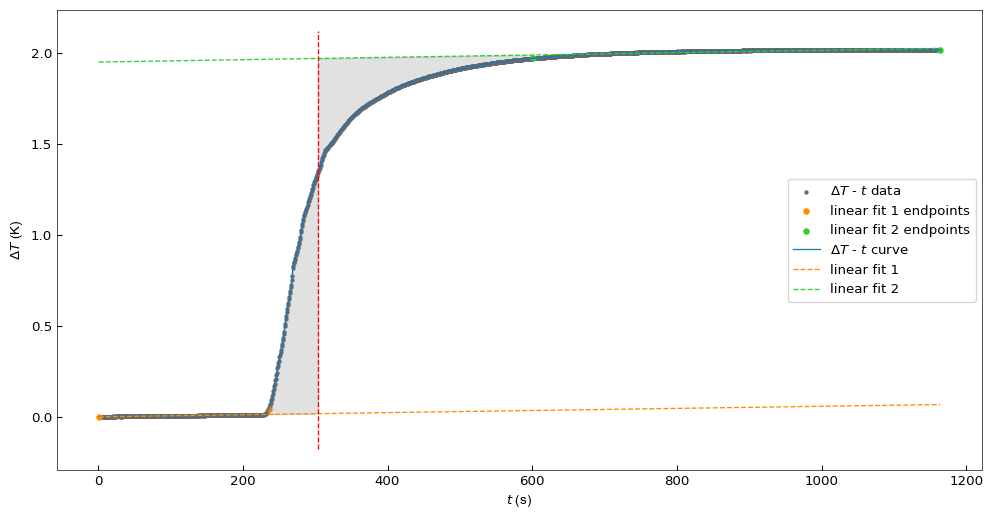
\includegraphics[width=0.9\textwidth]{4.png}
				\bicaption{单晶冰糖燃烧温差-时间关系}{The relationship between the temperature difference and time of rock candy combustion}
			\end{figure}
			由平台进行雷诺矫正后可知,燃烧前平台期温度 T1 = 0.0017 K,燃烧后平台期温度为 T2 = 1.973 K。因此燃烧前后的温差:
			\begin{equation}
				\Delta T = T_{2}-T_{1} = 1.973-0.0017 = 1.971\ \ {\rm K}
			\end{equation}
			单晶冰糖的恒容燃烧热$Q_{V}$可由下式求算:
			$$
			Q_{V}=-\frac{(W+DC_{\rm H_{2}O})\Delta T_{0}+\Sigma q}{G}
			$$
			\par
			其中,$\Delta T_{0}$为蔗糖燃烧使体系温度升高的数值$\Delta T_{0}=1.971\ \ {\rm ^{\circ}C}$;$G$为冰糖的质量,由2.2.3知$G=m-m^{\prime}=1.7091\ \ {\rm g}$;$D$为加入水的质量,由3.1.2知$D=2997\ \ {\rm g}$;$C_{\rm H_{2}O}$为水的比热容,由3.1.2知$C_{\rm H_{2}O}=4.184\ \ {\rm J\cdot g^{-1} \cdot K^{-1}}$;$W$为量热计常数,由3.1.2知$W=(2243\pm 96)\ \ {\rm J\cdot K^{-1}}$;$\Sigma q$为燃烧丝(镍丝)及棉线燃烧热的校正值,由2.2.3知棉线质量$m^{\prime}=0.0192\ \ {\rm g}$,发生燃烧的镍丝质量$m_{\rm Ni}=m_{0}-m_{1}=0.0053\ \ {\rm g}$,故计算:
			$$
			\Sigma q=Q_{V, {\rm Cotton}} \ \ m^{\prime}+Q_{V, {\rm Ni}} \ \ m_{\rm Ni}=(-16736\ \ {\rm J\cdot g^{-1}})\times 0.0192\ \ {\rm g}+(-3243\ \ {\rm J\cdot g^{-1}})\times 0.0053\ \ {\rm g}=-357\ \ {\rm J}
			$$
			\par
			根据以上各项数据,计算单晶冰糖的恒容燃烧热:
			$$
			Q_{V}=-\frac{(W+DC_{\rm H_{2}O})\Delta T_{0}+\Sigma q}{G}=-\frac{(2243\ \ {\rm J\cdot K^{-1}}+2.997\ \ {\rm kg}\times 4.184\ \ {\rm J\cdot g^{-1}\cdot K^{-1}})\times 1.971\ \ {\rm K}-357\ \ {\rm J}}{1.7091\ \ {\rm g}}
			$$
			$$
			=-1.684\times 10^{4}\ \ {\rm J\cdot g^{-1}}
			$$
			不确定度$\sigma_{Q_{V}}$由以下公式计算:
			$$
			\sigma_{Q_{V}}=\frac{1}{G}\sqrt{((W+DC_{\rm H_{2}O})\sigma_{\Delta T_{0}})^{2}+(\Delta T_{0}\sigma_{W})^{2}} \ \ {\rm J\cdot g^{-1}}
			$$
			$$
			=\frac{1}{1.7091\ \ {\rm g}}\sqrt{((2243\ \ {\rm J\cdot K^{-1}}+2.997\ \ {\rm kg}\times 4.184\ \ {\rm J\cdot g^{-1}\cdot K^{-1}})\times 0.001\ \ {\rm K})^{2}+(1.971\ \ {\rm K}\times 96\ \ {\rm J\cdot K^{-1}})^{2}}
			$$
			$$
			=70\ \ {\rm J\cdot g^{-1}}
			$$
			\par
			综上,测得单晶冰糖的恒容燃烧热为:
			$$
			Q_{V}=-(1.684\pm 0.070)\times 10^{4}\ \ {\rm J\cdot g^{-1}}
			$$
			冰糖本质就是白砂糖,其主要成分为蔗糖。蔗糖燃烧的反应方程式为:
			$$
			\ce{C12H22O11(s) +  12 O2(g) -> 12 CO2(g) + 11 H2O(l)}
			$$
			故$\Delta n=0$,冰糖的恒压燃烧热:
			$$
			Q_{P}=Q_{V}=-(1.684\pm 0.070)\times 10^{4}\ \ {\rm J\cdot g^{-1}}
			$$
			蔗糖的摩尔质量$M=342.30\ \ {\rm g\cdot mol^{-1}}$,故
			$$
			\Delta_{c}H_{m}=Q_{P}M=-(5764\pm 24)\ \ {\rm kJ\cdot mol^{-1}} 
			$$
			查阅\textit{CRC Handbook of Chemistry and Physics}\citealp{crc},知蔗糖的标准摩尔燃烧热
			$$
			\Delta_{c}H^{\circ}_{m}=-5640.9\ \ {\rm kJ\cdot mol^{-1}}
			$$
			故实验所测定的蔗糖燃烧热与文献参考值较为接近,相对误差为
			$$
			\xi=\frac{|\Delta_{c}H_{m}-\Delta_{c}H^{\circ}_{m}|}{\Delta_{c}H^{\circ}_{m}}\times 100\%=\frac{|-5764+5640.9|}{5640.9}\times 100\%=2.2\%
			$$
			\par
			推测存在偏差的原因为冰糖中除了蔗糖外还含有其他杂质,这些杂质的燃烧热可能与蔗糖的燃烧热不同,导致实验测得的燃烧热与文献参考值存在差异。\par

			
		\subsection{计算与推导}
		\subsubsection{利用 Origin 对蔗糖燃烧热进行雷诺校正}
		蔗糖燃烧热测定原始数据点过多,不利于 Origin 进行处理。从原始数据中,每 40组数据取一个点,所得数据如表 1 所示。\par
		\begin{table}[h]
			\centering
			\zihao{5}
			\bicaption{蔗糖燃烧过程体系温度变化实验数据}{Experimental data of temperature change of sucrose combustion process}
			\begin{tabular}{ccccccccccc}
				\arrayrulecolor{Maroon}
				\toprule
				$t/{\rm s}$ & $\Delta T/{\rm ^{\circ}C}$ & & $t/{\rm s}$ & $\Delta T/{\rm ^{\circ}C}$& & 	$t/{\rm s}$ & $\Delta T/{\rm ^{\circ}C}$ & & $t/{\rm s}$ & $\Delta T/{\rm ^{\circ}C}$ \\
				\midrule
				0.000   & 0.000  &  & 209.789 & -0.006 &  & 405.040 & 0.524 &  & 600.019 & 0.614 \\
				14.854  & -0.001 &  & 239.860 & -0.007&  & 417.225 & 0.540 &  & 630.902 & 0.618 \\
				29.937  & -0.003 &  & 269.252 & -0.007 &  & 435.195 & 0.553 &  & 660.799 & 0.621 \\
				44.917  & -0.005 &  & 282.412 & 0.002  &  & 450.891 & 0.563 &  & 690.165 & 0.623 \\
				59.851  & -0.006 &  & 299.985 & 0.080  &  & 465.129 & 0.572 &  & 720.559 & 0.626 \\
				75.333  & -0.005 &  & 315.487 & 0.219  &  & 479.411 & 0.580 &  & 750.020 & 0.628 \\
				89.638  & -0.006 &  & 330.520 & 0.322  &  & 493.943 & 0.586 &  & 780.629 & 0.628 \\
				104.926 & -0.006 &  & 346.668 & 0.397  &  & 509.357 & 0.592 &  & 810.413 & 0.628 \\
				118.814 & -0.005 &  & 360.677 & 0.445  &  & 525.902 & 0.597 &  &     &       \\
				149.132 & -0.005 &  & 375.438 & 0.483  &  & 540.266 & 0.601 &  &     &       \\
				179.764 & -0.005 &  & 390.320 & 0.506  &  & 570.609 & 0.607 &  &     &        \\
				\bottomrule
			\end{tabular}
		\end{table}
		\par
		使用 Origin 绘制燃烧过程温差-时间图,点间使用 B-样条连接,并通过雷诺校正对蔗糖燃烧过程的体系温度变化进行修正,如\textbf{图5}所示。
		\begin{figure}[!h]
			\centering
			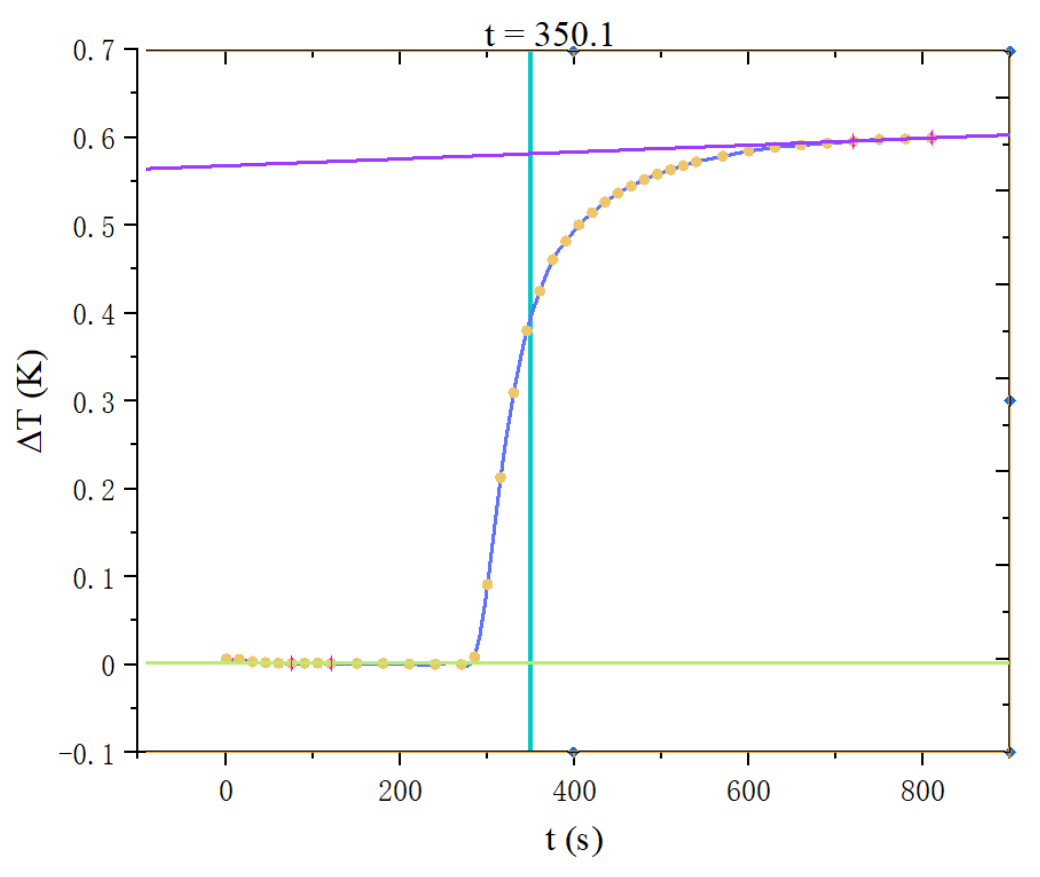
\includegraphics[width=0.7\textwidth]{5.png}
			\bicaption{蔗糖燃烧温差-时间关系(经雷诺校正)}{The relationship between the temperature difference and time of sucrose combustion}
		\end{figure}
		\par
		测定前期拟合直线的方程为:
		$$
		\Delta T/{\rm ^{\circ}C} =(1\pm 2)\times 10^{-6} \ \ t/{\rm s}-(9.5\pm 0.4)\times 10^{-4},\  \ R^{2}=0.9997
		$$
		测定末期拟合直线的方程为:
		$$
		\Delta T/{\rm ^{\circ}C} =(7.3\pm 1.4)\times 10^{-5} \ \ t/{\rm s}+(0.630\pm 0.01),\  \ R^{2}=0.9998
		$$
		确定使得两部分面积相等的时间点
		$$
		t_{0}=350.1\ \ {\rm s}
		$$
		计算垂线$t=t_{0}$与测定前期拟合直线的交点对应的温差
		$$
		\Delta T_{1}=-(0.0120\pm 0.0008)\ \ {\rm ^{\circ}C}
		$$
		计算垂线$t=t_{0}$与测定末期拟合直线的交点对应的温差
		$$
		\Delta T_{2}=(0.628\pm 0.01)\ \ {\rm ^{\circ}C}
		$$
		因此,计算蔗糖燃烧过程放出热量致使体系温度升高的数值
		$$
		\Delta T_{0}=(0.630\pm 0.01)\ \ {\rm ^{\circ}C}
		$$
		\par
		由此可计算蔗糖的恒容燃烧热:
		$$
		Q_{V}=-\frac{(W+DC_{\rm H_{2}O})\Delta T_{0}+\Sigma q}{G}
		$$
		$$
		=-\frac{(2243\ \ {\rm J\cdot K^{-1}}+2.997\ \ {\rm kg}\times 4.184\ \ {\rm J\cdot g^{-1}\cdot K^{-1}})\times 0.630\ \ {\rm K}-442\ \ {\rm J}}{0.5769\ \ {\rm g}}
		$$
		$$
		=-15380\ \ {\rm J\cdot g^{-1}}
		$$
		\par
		不确定度$\sigma_{Q_{V}}$由以下公式计算:
		$$
		\sigma_{Q_{V}}=\frac{1}{G}\sqrt{((W+DC_{\rm H_{2}O})\sigma_{\Delta T_{0}})^{2}+(\Delta T_{0}\sigma_{W})^{2}} \ \ {\rm J\cdot g^{-1}}
		$$
		$$
		=\frac{1}{0.5769\ \ {\rm g}}\sqrt{((2243\ \ {\rm J\cdot K^{-1}}+2.997\ \ {\rm kg}\times 4.184\ \ {\rm J\cdot g^{-1}\cdot K^{-1}})\times 0.001\ \ {\rm K})^{2}+(0.630\ \ {\rm K}\times 96\ \ {\rm J\cdot K^{-1}})^{2}}
		$$
		$$
		=107\ \ {\rm J\cdot g^{-1}}
		$$
		蔗糖的恒压燃烧热:
		$$
		Q_{P}=Q_{V}=-(1.538\pm 0.107)\times 10^{4}\ \ {\rm J\cdot g^{-1}}
		$$
		蔗糖的摩尔质量$M=342.30\ \ {\rm g\cdot mol^{-1}}$,故
		$$
		\Delta_{c}H_{m}=Q_{P}M=-(5664\pm 24)\ \ {\rm kJ\cdot mol^{-1}}
		$$
		查阅\textit{CRC Handbook of Chemistry and Physics}\citealp{crc},知蔗糖的标准摩尔燃烧热
		$$
		\Delta_{c}H^{\circ}_{m}=-5640.9\ \ {\rm kJ\cdot mol^{-1}}
		$$
		故实验所测定的蔗糖燃烧热与文献参考值较为接近,相对误差为:
		$$
		\xi=\frac{|\Delta_{c}H_{m}-\Delta_{c}H^{\circ}_{m}|}{\Delta_{c}H^{\circ}_{m}}\times 100\%=\frac{|-5664+5640.9|}{5640.9}\times 100\%=0.4\%
		$$


 	\section{讨论与结论}
 		\subsection{实验结论}
		 本实验通过氧弹式量热计中苯甲酸、蔗糖和单晶冰糖的恒容燃烧,经雷诺校正及热力学计算得到量热计常数$W=(2.243\pm 0.097)\ \ {\rm kJ\cdot K^{-1}}$,单晶冰糖的恒压燃烧热$Q_{V}=-(1.684\pm 0.070)\times 10^{4}\ \ {\rm kJ\cdot g^{-1}}$,恒容燃烧热$Q_{P}=-(1.684\pm 0.070)\times 10^{4}\ \ {\rm kJ\cdot g^{-1}}$,与文献值的偏差$\xi=2.2\%$,使用 Origin 软件进行雷诺校正,测得样品白方糖燃烧热$Q_{P}=Q_{V}=-(1.538\pm 0.107)\times 10^{4}\ \ {\rm kJ\cdot g^{-1}}$。

\vbox{}  
%参考文献
\bibliographystyle{unsrt}
\bibliography{cite}
\end{document}